% Asset ID: AS1DifferentiationTIKZ-008
% Source: CCEA AS1-DIFF-LO003 + Chapter 12 rate-of-change evidence
% Related lesson section: Core Theory 23
% Purpose: Connect dV/dt with volume changing over time.

\documentclass[tikz,border=8pt]{standalone}
\usepackage{amsmath}
\usepackage{pgfplots}
\usetikzlibrary{arrows.meta}
\pgfplotsset{compat=1.18}

\begin{document}
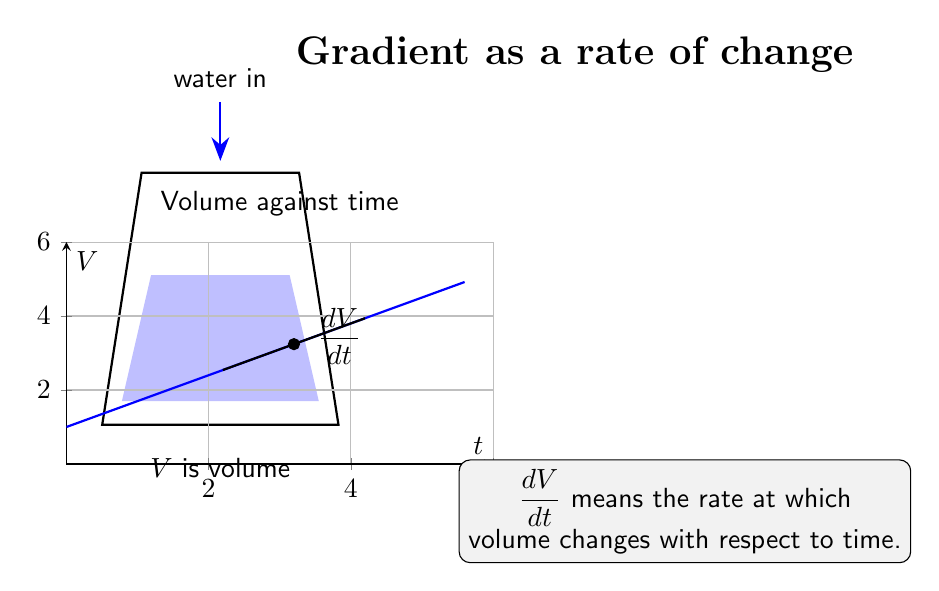
\begin{tikzpicture}[font=\sffamily, >=Stealth]

\node[font=\Large\bfseries] at (6.5,5.2) {Gradient as a rate of change};

\draw[thick] (0.5,0.5) -- (1,3.7) -- (3,3.7) -- (3.5,0.5) -- cycle;
\fill[blue!25] (0.75,0.8) -- (1.12,2.4) -- (2.88,2.4) -- (3.25,0.8) -- cycle;
\draw[blue, thick, -{Stealth[length=3mm]}] (2,4.6) -- (2,3.85);
\node at (2,4.9) {water in};
\node at (2,-0.05) {$V$ is volume};

\begin{axis}[
    at={(5,0.2)},
    width=7cm,
    height=4.4cm,
    axis lines=middle,
    xmin=0, xmax=6,
    ymin=0, ymax=6,
    xlabel={$t$},
    ylabel={$V$},
    grid=both,
    title={Volume against time},
    samples=100,
    domain=0:5.6
]
\addplot[blue, thick] {0.7*x + 1};
\addplot[black, thick, domain=2.2:4.2] {0.7*x + 1};
\addplot[only marks, mark=*, black] coordinates {(3.2,3.24)};
\node[anchor=west] at (axis cs:3.4,3.45) {$\displaystyle \frac{dV}{dt}$};
\end{axis}

\node[draw, rounded corners, fill=gray!10, align=center] at (7.9,-0.6)
{$\displaystyle \frac{dV}{dt}$ means the rate at which\\volume changes with respect to time.};

\end{tikzpicture}
\end{document}
